\section{Existing bone conductor}
The chose for a \gls{bc} require knowledge of existing \gls{bc} and vibrators of possible \gls{bc} for the purpose of this project. Therefore this section will analyse the most common \gls{bc} for hearing damage test and analyse different kind of vibrators founded by research. 

\subsection{B71}
One of the most widely used \gls{bc} is the Radioear Corporation B71, which build on the electromagnetic transducers of the variable reluctance type. The benefit for using such type of transducer is that the transducer have a wide frequency response, high impedance and efficiency in a small size packed. The principle of the variable reluctance type is that it function according to the horseshoe magnet principle. This principle means that there is a small air gab between the yoke, which is attached to the outer plastic cabinet of the B71, and the armature which basically is the permanent magnet. \citep{the_balanced_2003}. The force in the air gap, between the yoke and the armature can be changed by generate a magnetic field in the coil which make the armature to move. This force change and movement will make vibration and vibrate accordingly to the input signal. To transfer acoustic signal to the skull, the transducer is required to be pressed to the skull with a minimum force of \SI{5}{\newton}. At hearing test the transducer shall be pressed against the mastoid area behind the ear with the earlier mentioned force. 


 The following \autoref{fig:r_b71} shows a inside cut for the B71.

 \begin{figure}[H]
	\centering
		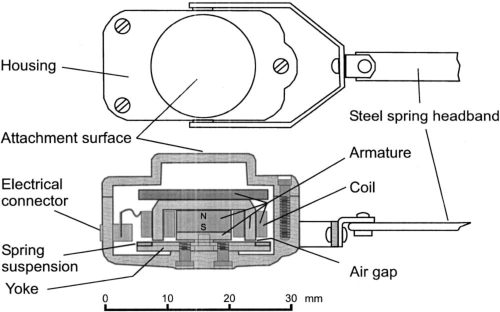
\includegraphics[width=1\textwidth]{r_b71}
		\caption{The figure shows a cross-section cut of the Radioear Corporation B71  \citep{the_balanced_2003}.}
		\label{fig:r_b71}
\end{figure}

The design of the B71 have limits which make it poor for music and communication use. The transducer have high distortion in frequency below \SI{1}{\kilo\hertz} and goes to approximate \SI{61}{\percent} distortion at \SI{250}{\hertz}. Furthermore the transducer have poor frequency response. The first-order analysis of the electromagnetic circuit is explained in this article \autoref{fig:r_b71}. The conclusion for this kind of magnetic circuit is that it require a high static magnetic force and therefore a stiff suspension to avoid collapse of the air gap. A transducer is normally designed such that the resonance frequency of the transducer lays slightly above the lowest frequency for the transducer. With respect to the resonance formula of the circuit for B71, only the mass of the counterweight for the transducer or the stiffness for the suspension can be changed to get a better low frequency response. The formula is as following \autoref{eq:res_b71} \autoref{fig:r_b71}.

\begin{equation}\label{eq:res_b71}
f_r=\frac{1}{2 \pi \sqrt{m C}}
\end{equation}

    \startexplain
    		\explain{$f_r$ is the resonance frequency }{\si{\hertz}}
        \explain{$m$ is the mass of the counterweight}{\si{\kilo\gram}}
        \explain{$C$ is the compliance of the suspension}{\si{.(\newton\per\meter)^{-1}}}
    \stopexplain

The \autoref{eq:res_b71} explain well that ether the mass has to be bigger or the compliance have to be higher. By doing the compliance higher the stiffness suffer and the air gab can not be maintained and therefore only the mass can be changed. Raising the mass of the counterweight makes the transducer bigger and the weight will rise. To avoid a bigger and more heavy design, the Radioear Corporation B81 have been designed and will be explained next. 


\subsection{B81}
The Radioear Corporation B81 is building on the \gls{best} principle.

https://pdfs.semanticscholar.org/9407/bf610cf2fc32835a5ca07dcce3d4b4b08599.pdf?_ga=2.147405172.291536821.1537166972-1605440078.1536836079